\begin{frame}{Latent and observed variables}
  \begin{itemize}
    \item Structural equation models consist of \emph{latent} and \emph{observed} variables
    \item An observed variable is one that come from outside the model---like a survey question
    \item A latent variable is a variable that is determined inside the model---like an attitudinal factor
    \item Every model has observed variables, some don't have latent variables
  \end{itemize}
\end{frame}

\begin{frame}{Exogenous and endogenous variables}
  \begin{itemize}
    \item An \emph{exogenous} variable is one that is not influenced by any other variable in the model
    \begin{itemize}
      \item \textit{i.e.} no arrows pointing to the variable
    \end{itemize}
    \item An \emph{endogenous} variable is a variable that is influenced by at least one other variable in the model
    \begin{itemize}
      \item \textit{i.e.} at least one arrow pointing to the variable
      \item there may or may not be arrows pointing away from the variable
    \end{itemize}
    \item All SEMs have at least one endogenous variable, almost all have exogenous variables
  \end{itemize}
\end{frame}

\begin{frame}{Latent and observed vs. endogenous and exogenous variables}
  \begin{itemize}
    \item Latent and observed have nothing to do with endogenous or exogenous
    \item All of these types of variables are possible
    \begin{itemize}
      \item observed, endogenous
      \item latent, endogenous
      \item observed, exogenous
      \item latent, exogenous
    \end{itemize}
  \end{itemize}
\end{frame}

\begin{frame}{Exploratory factor analysis, confirmatory factor analysis, and SEMs}
  \begin{itemize}
    \item Exploratory factor analysis is a separate method from SEMs
    \item Confirmatory factor analysis can be (and usually is) \emph{part of} the SEM
    \item Most authors use an exploratory factor analysis to identify the structure before using a confirmatory factor analysis in their SEM
  \end{itemize}
\end{frame}

\begin{frame}{Confirmatory factor analysis in an SEM}
  \small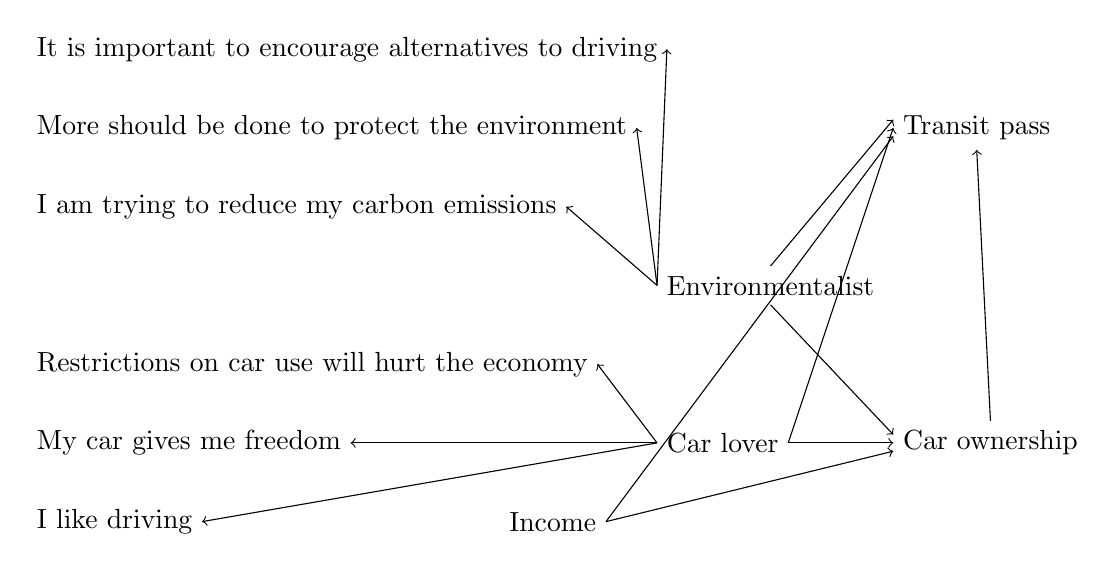
\begin{tikzpicture}
    \node[anchor=west,text=black] (likedriving) at (0, 0) {I like driving};
    \node[anchor=west,text=black] (carfreedom) at (0, 1) {My car gives me freedom};
    \node[anchor=west,text=black] (careconomy) at (0, 2) {Restrictions on car use will hurt the economy};

    \node[anchor=west,text=black] (carbon) at (0, 4) {I am trying to reduce my carbon emissions};
    \node[anchor=west,text=black] (protect) at (0, 5) {More should be done to protect the environment};
    \node[anchor=west,text=black] (alt) at (0, 6) {It is important to encourage alternatives to driving};

    \node[anchor=west,text=black] (carlover) at (8, 1) {Car lover};
    \node[anchor=west,text=black] (env) at (8, 3) {Environmentalist};

    \node[anchor=west,text=black] (carownership) at (11, 1) {Car ownership};
    \node[anchor=west,text=black] (tpass) at (11, 5) {Transit pass};

    \node[anchor=west,text=black] (inc) at (6, 0) {Income};

    \draw[black,<-] (likedriving.east) -- (carlover.west);
    \draw[black,<-] (carfreedom.east) -- (carlover.west);
    \draw[black,<-] (careconomy.east) -- (carlover.west);

    \draw[black,<-] (carbon.east) -- (env.west);
    \draw[black,<-] (protect.east) -- (env.west);
    \draw[black,<-] (alt.east) -- (env.west);

    \draw[->] (env.south) -- ([yshift=0.3em]carownership.west);
    \draw[->] (carlover.east) -- (carownership.west);
    \draw[->] (env.north) -- ([yshift=0.3em]tpass.west);
    \draw[->] (carlover.east) -- (tpass.west);

    \draw[->] (inc.east) -- ([yshift=-0.3em]carownership.west);
    \draw[->] (inc.east) -- ([yshift=-0.3em]tpass.west);

    \draw[->] (carownership.north) -- (tpass.south);
  \end{tikzpicture}
\end{frame}

\begin{frame}{Confirmatory factor analysis in an SEM}
  \small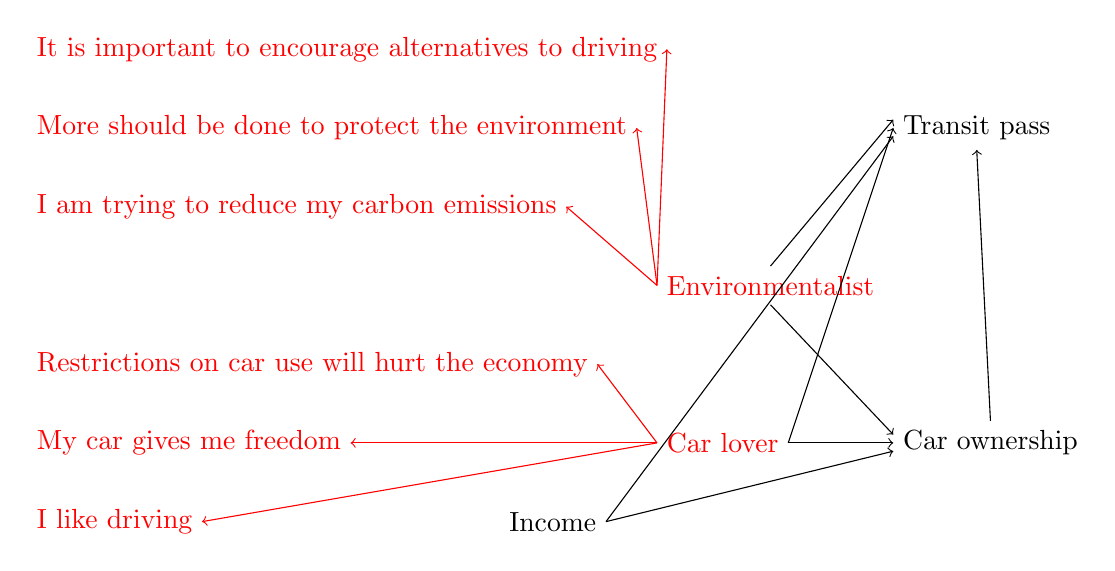
\begin{tikzpicture}
    \node[anchor=west,text=red] (likedriving) at (0, 0) {I like driving};
    \node[anchor=west,text=red] (carfreedom) at (0, 1) {My car gives me freedom};
    \node[anchor=west,text=red] (careconomy) at (0, 2) {Restrictions on car use will hurt the economy};

    \node[anchor=west,text=red] (carbon) at (0, 4) {I am trying to reduce my carbon emissions};
    \node[anchor=west,text=red] (protect) at (0, 5) {More should be done to protect the environment};
    \node[anchor=west,text=red] (alt) at (0, 6) {It is important to encourage alternatives to driving};

    \node[anchor=west,text=red] (carlover) at (8, 1) {Car lover};
    \node[anchor=west,text=red] (env) at (8, 3) {Environmentalist};

    \node[anchor=west,text=black] (carownership) at (11, 1) {Car ownership};
    \node[anchor=west,text=black] (tpass) at (11, 5) {Transit pass};

    \node[anchor=west,text=black] (inc) at (6, 0) {Income};

    \draw[red,<-] (likedriving.east) -- (carlover.west);
    \draw[red,<-] (carfreedom.east) -- (carlover.west);
    \draw[red,<-] (careconomy.east) -- (carlover.west);

    \draw[red,<-] (carbon.east) -- (env.west);
    \draw[red,<-] (protect.east) -- (env.west);
    \draw[red,<-] (alt.east) -- (env.west);

    \draw[->] (env.south) -- ([yshift=0.3em]carownership.west);
    \draw[->] (carlover.east) -- (carownership.west);
    \draw[->] (env.north) -- ([yshift=0.3em]tpass.west);
    \draw[->] (carlover.east) -- (tpass.west);

    \draw[->] (inc.east) -- ([yshift=-0.3em]carownership.west);
    \draw[->] (inc.east) -- ([yshift=-0.3em]tpass.west);

    \draw[->] (carownership.north) -- (tpass.south);
  \end{tikzpicture}
\end{frame}

\begin{frame}<1>{Exploratory factor analysis in an SEM}
  \small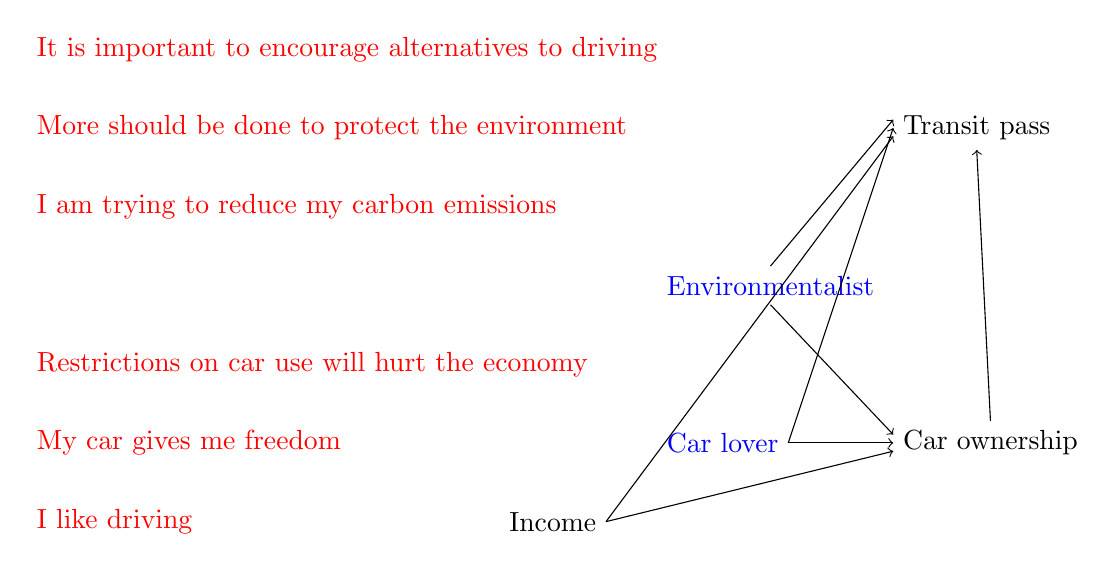
\begin{tikzpicture}
    \onslide<2>{
    \node[anchor=west,text=red] (likedriving) at (0, 0) {I like driving};
    \node[anchor=west,text=red] (carfreedom) at (0, 1) {My car gives me freedom};
    \node[anchor=west,text=red] (careconomy) at (0, 2) {Restrictions on car use will hurt the economy};

    \node[anchor=west,text=red] (carbon) at (0, 4) {I am trying to reduce my carbon emissions};
    \node[anchor=west,text=red] (protect) at (0, 5) {More should be done to protect the environment};
    \node[anchor=west,text=red] (alt) at (0, 6) {It is important to encourage alternatives to driving};
    }

    \node[anchor=west,text=blue] (carlover) at (8, 1) {Car lover};
    \node[anchor=west,text=blue] (env) at (8, 3) {Environmentalist};

    \node[anchor=west,text=black] (carownership) at (11, 1) {Car ownership};
    \node[anchor=west,text=black] (tpass) at (11, 5) {Transit pass};

    \node[anchor=west,text=black] (inc) at (6, 0) {Income};

    \draw[->] (env.south) -- ([yshift=0.3em]carownership.west);
    \draw[->] (carlover.east) -- (carownership.west);
    \draw[->] (env.north) -- ([yshift=0.3em]tpass.west);
    \draw[->] (carlover.east) -- (tpass.west);

    \draw[->] (inc.east) -- ([yshift=-0.3em]carownership.west);
    \draw[->] (inc.east) -- ([yshift=-0.3em]tpass.west);

    \draw[->] (carownership.north) -- (tpass.south);
  \end{tikzpicture}
\end{frame}

\begin{frame}{Exploratory factor analysis in an SEM}
  \begin{itemize}
    \item If factors are found with an exploratory factor analysis, there are calculated before the SEM is fit
    \item Thus, from the perspective of the SEM, these are \emph{observed} variables
    \item ...even though they were latent variables in the exploratory factor analysis
    \pause\item (but not everyone agrees with me on this)
  \end{itemize}
\end{frame}
